% TODO: Длинные заголовки при переносе строки продолжаются под цифрами. Т.е. не начало текста не выровнено
% ----------------------------- БАЗОВЫЕ НАСТРОЙКИ  -----------------------------

\documentclass[oneside, final, 14pt,  a4paper]{extreport}    % Класс документа. Чаще всего использует его
\usepackage[T2A]{fontenc}
\usepackage[utf8]{inputenc}                        % Кодировка utf8x для linux
\usepackage[english,russian]{babel}                % Переносы и прочее для русского и английского
\usepackage[linktocpage=true]{hyperref}            % Гиперссылки
\usepackage{indentfirst}                           % Красная строка для первых абзацев
\usepackage{mathtools}
\usepackage{tabularx}                              % Много табличной боли и магии
%\usepackage{ltablex}                              % Длинные таблицы с разрывом страниц
%\keepXColumns                                     % Чтобы ltablex не ломал ширину
\usepackage{tabulary}                              % Для создания выравненных "где..." для формул
\usepackage{graphicx}
\usepackage{titlesec}                              % Для настройки названий глав, разделов итп
\usepackage{titletoc}                              % Для настройки оглавления
\usepackage{enumitem}                              % Для настройки списков
\usepackage{flafter}                               % Плавающие элементы встречаются после ссылки на них
\usepackage{caption}                               % Настройка подписей плавающих элементов
\usepackage{setspace}                              % Для настройки интервалов
\usepackage{color, soulutf8}                       % Выделенный текст
\usepackage{csquotes}
\usepackage{algorithm}                             % Псевдокод
\usepackage{algpseudocode}
\usepackage{chngcntr}                              % Чтоб настроить сквозную нумерацию
\usepackage{lastpage}                              % Получить количество страниц
\usepackage[figure,table]{totalcount}              % Получить количество рисунков и таблиц

% Библиография
\usepackage[
    backend=biber,
    sorting=none,                                  % Сортировка в порядке цитирования
	style=gost-numeric,
	language=auto,                                 % Автовыбор стиля, напр. писать [et al] вместо [и др]
	autolang=other                                 % для англоязычных публикаций (langid={english})
] {biblatex}

\linespread{1.3}                                   % Полуторный интервал

% Настройка полей
\usepackage{geometry}
\geometry{left=3cm}
\geometry{right=1cm}
\geometry{top=1.5cm}
\geometry{bottom=2cm}


\sloppy                                           % Избегать залезания строк на поля (надо?)
\setlength\parindent{1.5cm}                       % Отступ красной строки

\newcommand{\nf}{\normalfont}

% Для tabularx: как X (растянутый), только выравненный по центру
\newcolumntype{Y}{>{\centering\arraybackslash}X}
\newcolumntype{P}{>{\raggedleft\arraybackslash}X}

%--------------------------- НАСТРОЙКА ТИТУЛЬНОГО ЛИСТА ------------------------
\newenvironment{nospasing}
{
    \begin{spacing}{1}
}
{
    \end{spacing}
}

% Поля титульного листа с подписями и линями (подпись, ФИО итп)

% подпись под пустой линией заданной длины
\newcommand{\efield}[2][2cm]{
	%1 - ширина поля
	%2 - подпись под линией
	$\underset{\text{(#2)}}{\underline{\hspace*{#1}}}$
}

% Подпись под текстом
\newcommand{\tfield}[2]{
	%1 - содержимое поля
	%2 - подпись под линией
	$\underset{\text{(#2)}}{\underline{\smash{\text{#1}}}}$
}

% Название поля, линия до конца строки, значение поля над линией, подпись под линией

\newcommand{\lfield}[3]{
	%1 - название поля
	%2 - содержимое поля
	%3 - подпись под линией
	\noindent
	\renewcommand{\arraystretch}{0.7}
	\begin{tabularx}{\linewidth}{@{}lY@{}}
    	#1 & #2 \\
    	\cline{2-2}
           & \footnotesize(#3)\normalsize
	\end{tabularx}

}


% ----------------------------- НАСТРОЙКИ ЗАГЛАВИЙ -----------------------------
%% Отступ 1.5 слева (как у красной строки)t
% Нет точки между номером и названием
% Интервал между подзаголовками 1.5
% Интервал между заголовком и текстом 2*1.5
% Поддержка приложений

% Глава
\titleformat{\chapter}
	[block]                % Shape. block убирает перенос заглвания на новую строку
    {\normalfont}          % Format. Собственно, стиль
    {\thechapter}          % Label. Номер главы.
    {8pt}                  % Sep. Пробел между номером и главой (TODO: уточнить)
    {}                     % before-code. Код перед названием
\titlespacing*{\chapter}
	{1.5cm}                % Левый отступ (как у красной строки)
	{18pt}                 % Верхний отступ, 1.5 интервал
	{18pt}                 % Нижний отступ, 1.5 интервал

% Раздел
\titleformat{\section}
	{\normalfont}
	{\thesection}
	{8pt}{}
\titlespacing*{\section}
	{1.5cm}{18pt}{18pt}

% Подраздел
\titleformat{\subsection}
	{\normalfont}
	{\thesubsection}
	{8pt}{}
\titlespacing*{\subsection}
	{\parindent}{18pt}{18pt}

% Глава без номера (введение, заключение и т.п.)
\newcommand{\nnchapter}[1]
{
	\chapter*{#1}
	\addcontentsline{toc}{chapter}{#1}
}

% Фейковая глава для автореферата
% Зачем платить больше, если не нужно содержание?
\newcommand{\referchapter}[1]
{

    \vspace{18pt}
    #1
    \vspace{18pt}

}


% Приложения
% Использовать \chapter{} для создания приложений
% Очень грязный хак, но работает
\newcommand{\StartAppendix}
{
	\setcounter{chapter}{0}
}

\renewcommand{\appendix}[1]
{
	\newpage
	\stepcounter{chapter}
	\newcommand{\theappendix}{ПРИЛОЖЕНИЕ \MakeUppercase{\asbuk{chapter}}}
	\addcontentsline{toc}{chapter}{\texorpdfstring{\theappendix} ~--- #1}
	\begin{center}
		\theappendix\\
		{#1}
	\end{center}
}

% Расстояние между заглавиями и текстом должно быть 2 полуторных интервала,
% а расстояние между заглавиями - один полуторный интервал.
% Не придумал ничего лучше, кроме как вставлять вручную
\newcommand{\aftertitle}{\vskip 18pt}

% ----------------------------- НАСТРОЙКИ СОДЕРЖАНИЯ ---------------------------
% Нет выделения жирным
% Все с одним уровнем отступа
% Поддержка приложений

% Главы
\titlecontents{chapter}
	[0em] {}
	{\thecontentslabel~}{}
	{\titlerule*[1pc]{.}\contentspage}

% Разделы
\titlecontents{section}
	[0em] {}
	{\thecontentslabel~}{}
	{\titlerule*[1pc]{.}\contentspage}

% Подразделы
\titlecontents{subsection}
	[0em] {}
	{\thecontentslabel~}{}
	{\titlerule*[1pc]{.}\contentspage}

% Заголовок
\addto\captionsrussian{
	\renewcommand{\contentsname} {СОДЕРЖАНИЕ}
}

%-------------------------------- НАСТРОЙКИ СПИСКОВ ----------------------------
% Маркерный список
\setlist[itemize]{
	label=-,                  % Дефис в каяестве маркера
	leftmargin=1.5cm,         % Текст в списке выравнен по красной строке
	itemindent=15pt,          % Маркер выравнен по красной строке, т.е. первая строка чуть сдвинута на размер маркера
	nosep                     % Убираем интервал между пунктами списков
}

% Числовой
\setlist[enumerate]{
    label*=\arabic*),
    leftmargin=1.5cm,
    itemindent=15pt,
    nosep
}

%--------------------------- НАСТРОЙКИ РИСУНКОВ И ТАБЛИЦ -----------------------
% Рисунки подписываются "Рисунок N - ..." по центру
% Таблицы подписываются "Таблица N - ..." с левого края

\captionsetup[figure]{
	name=Рисунок,
	labelsep=endash,
	justification=centering,
	belowskip=-17pt,aboveskip=0pt,
	font={stretch=1.3}
}
\captionsetup[table]{name=Таблица, labelsep=endash, justification=raggedright, singlelinecheck=false}

% Сквозная нумерация таблиц, рисунков и формул
\counterwithout{figure}{chapter}
\counterwithout{table}{chapter}
\counterwithout{equation}{chapter}
\pdfimageresolution=150

%\setlength{\belowcaptionskip}{-14pt}

%---------------------------------- ФОРМУЛЫ ------------------------------------

\newcommand{\degsym}{^{\circ}}    % Градус
\newcommand{\CST}{\mathcal{C}}    % C-State, пространство конфигурации
\newcommand{\XST}{\mathcal{X}}    % X-State, пространство состояний
\newcommand{\vect}[1]{\overrightarrow{#1}}
\DeclarePairedDelimiter\floor{\lfloor}{\rfloor}

%-------------------------------- БИБЛИОГРАФИЯ ---------------------------------

\addbibresource{autonomouscar.bib}
\begin{document}

% Выключить нумерацию на титульной странице
\thispagestyle{empty}

\begin{nospasing}
\begin{center}
    Министерство образования и науки Российской Федерации \\
    Федеральное государственное бюджетное образовательное учреждение \\
    высшего образования \\
    «Волгоградский государственный технический университет» \\
    Факультет электроники и вычислительной техники \\
    Кафедра «Электронно-вычислительные машины и системы» \\

    \begin{flushright}
    На правах рукописи \\
    \end{flushright}

    МАРКОВ АЛЕКСЕЙ ЕВГЕНЬЕВИЧ \\
    \vspace{1cm}
    Разработка метода построения программной траектории и регулятора движения по ней беспилотного
    наземного транспортного средства \\
    \vspace{1cm}
    Магистерская программа \\
    «Высокопроизводительные вычислительные системы» \\
    Направление подготовки 09.04.01 «Информатика и вычислительная техника» \\
    \vspace{1cm}
    АВТОРЕФЕРАТ \\
    \vspace{1cm}
    диссертации на соискание степени \\
    магистра \\

    \vfill

    Волгоград – 2019
\end{center}
\end{nospasing}

\newpage

\begin{nospasing}
\noindent
Работа выполнена на кафедре «Электронно-вычислительные машины и
системы» Волгоградского государственного технического университета\\

\noindent
Научный руководитель:\\

    \setlength{\leftskip}{3cm}
    \noindent
    доктор технических наук, \\
    профессор Горобцов Александр Сергеевич \\

    \setlength{\leftskip}{0pt}

\noindent
Рецензент:

    \setlength{\leftskip}{3cm}
    \noindent
    \hl{TODO} \\

    \setlength{\leftskip}{0pt}

\end{nospasing}

\newpage

%%%%%%%%%%%%%%%%%%%%%%%%%%%%%%%%%%%%%%%%%%%%%%%%%%%%%%%%%%%%%%%%%%%%%%%%%%%%%%

\referchapter{ОБЩАЯ ХАРАКТЕРИСТИКА РАБОТЫ}
\textbf{Актуальность темы исследования.}

Использование беспилотных систем и интеллектуальных систем помощи водителю (ADAS) на дорогах общего
пользования приведет к повышению безопасности дорожного движения по причине уменьшения человеческого
фактора, увеличению пропускной способности дорог и дорожной инфраструктуры, уменьшению пробок, а также
уменьшить количество личных автомобилей при сохранении текущих сценариев использования, что еще
сильнее снизит нагрузку на инфраструктуру и загрязнение окружающей среды.

На кафедрах ЭВМиС, ВМ и АТ ВолгГТУ в настоящее время ведется разработка прототипа беспилотного
автомобиля на базе автомобиля Лада Калина.

\textbf{Цель и задачи работы.}

Целью данной работы является разработка метода построения программной траектории и регулятора движения по ней
беспилотного наземного транспортного средства.
Для достижения данной цели решались следующие задачи:
\begin{enumerate}
    \item анализ существующих подходов к задаче управления беспилотными автомобилями в целом, выделение
          типичных подсистем, анализ методов планирования движения для наземных транспортных средств;
    \item проектирование и реализация подсистемы формирования программной траектории;
    \item проектирование и реализация подсистемы движения по траектории,
    \item проведение экспериментов и оценка результатов работы.
\end{enumerate}

\textbf{Объектом исследования является} процесс управления движением беспилотного автомобиля.

\textbf{Предметом исследования являются} алгоритмы и подходы к реализации системы управления движением
беспилотного наземного транспортного средства.

\textbf{Основные положения, выносимые на защиту:}
\begin{enumerate}
    \item подход к построению программной траектории для беспилотного транспортного средства, совмещающий метод
          интерполяции кривыми с поиском кратчайшего пути на графе,
    \item разработанная архитектура системы управления беспилотным наземным транспортным средством.
\end{enumerate}

\textbf{Научной новизной} работы является
\begin{enumerate}
    \item был разработан алгоритм построения программной траектории для наземного беспилотного транспортного
          средства, осуществляющий построение траектории в форме полиномов пятого порядка, отличающийся от существующего
          добавлением поиском кратчайшего пути на графе состояний, что позволяет осуществлять планирование на несколько
          шагов вперед;
    \item был разработан регулятор для движения по программной траектории с использованием обратной связи
          от системы SLAM.
\end{enumerate}

\textbf{Практическая ценность} работы заключается в реализации системы построения программной
траектории и движения по ней беспилотного наземного транспортного средства.

\textbf{Апробация} работы проводилась на ряде конференций и выставок.

\textbf{Публикации.} По материалам диссертации автором были опубликованы две работы.

\textbf{Структура и объем работы}. Диссертационная работа состоит из введения, четырех глав, заключения,
списка использованных источников из 56 наименований и насчитывает 95 страниц, в том числе 35
рисунков и 2 таблицы.

\referchapter{ОСНОВНОЕ СОДЕРЖАНИЕ РАБОТЫ}
\textbf{Во введении} обосновывается выбор темы диссертационного исследования и ее актуальность,
определяются цели и задачи работы, объект и предмет исследования, формулируется научная новизна.

\textbf{В первой главе} анализируется типичный применяемый подход к построению систем управления
беспилотными автомобиля и применяемые методы планирования движения. Анализируя источники по данной тематике,
можно сделать вывод, что, несмотря на большое количество архитектур систем управления беспилотными
автомобилями, можно выделить общие архитектурные концепции (рисунок \ref{img:general_arch}).

В общем виде, систему управления беспилотным автомобилем
можно разделить на следующие подсистемы:
\begin{itemize}
    \item интерфейс сенсоров, позволяющий получать данные от сенсоров;
    \item подсистема восприятия (perception), осуществляющая построение комплексной информации об
    окружающем пространстве, на основе данных от сенсоров;
    \item подсистема управления движением,осуществляющая принятие решений и построение безопасной
    и достижимой траектории и осуществляющая движение по траектории, формирования управляющих сигналов,
    таких как угол поворота руля, газ, тормоз.
\end{itemize}

\begin{figure}[h]
    \centering
    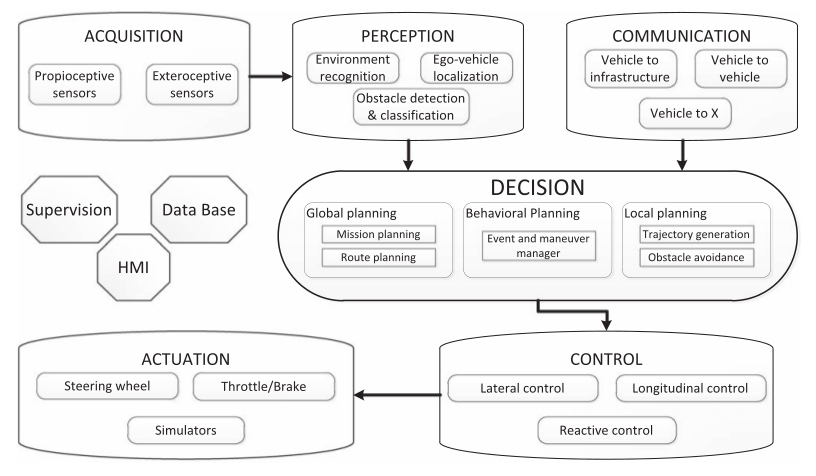
\includegraphics[width=\linewidth]{images/general_arch}
    \caption{Обобщенная абстракция архитектуры управления автономными автомобилями}
    \label{img:general_arch}
\end{figure}

Процесс планирования движения и принятия решений в современных беспилотных автомобилях обычно представлен в виде
иерархии: планирование маршрута (route planning), принятие решений (behaviour planning, decision making), локально планирование
(local motion planning) и управление с обратной связью.

На верхнем уровне осуществляется планирование маршрута по дорожной сети. Затем следуют уровень планирования
поведения, который принимает решения и формирует локальные навигационные задачи, которые приближают автомобиль
к выполнению высокоуровневой задачи и удовлетворяют правилам дорожного движения. Затем локальный планировщик
формирует непрерывный кинематически и динамически достижимый путь в обход препятствий в окружающем пространстве, который выполняет локальную навигационную задачу. Система
управления с обратной связью осуществляет выполнение запланированного движения и коррекцию ошибок.

В данной работе основной акцент делается на планировании локального движения. Рассматривается ряд распространенных
методов планирования движения: метод планирования на графах, в частности, метод клеточной декомпозиции, случайные
(sample-based) методы, основанные на алгоритме Rapidly Exploring Random Trees (RRT) и его модификациях, методы
интерполяции траектории с помощью кривых.

\textbf{Во второй главе} рассматривается проектирование системы управления движением беспилотного автомобиля.

Для планирования локальной траектории траектории выбран метод интерполяции кривыми, а именно, полиномами
пятого порядка. Метод интерполяции выбран по причине его детерминированности и возможности находить оптимальное
или близкое к нему решение.

Планирование траектории осуществляется в подвижной системе координат, образованной репером Френе,
движущейся по идеальной траектории, как показано на рисунке \ref{img:junior_frenet_frame}. В качестве
идеальной траектории  выступает центр полосы движения. Это является распространенным подходом к
планированию движения и позволяет рассмотреть независимо планирование поперечного движения и
продольного движения (профиля скорости).

\begin{figure}[h]
    \centering
    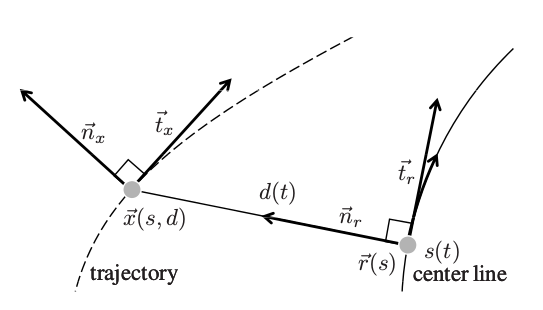
\includegraphics[width=0.7\textwidth]{images/junior_frenet_frame}
    \caption{Система координат для планирование траектории}
    \label{img:junior_frenet_frame}
\end{figure}

Для нахождения оптимальной траектории, определена функция стоимости, основанная на минимизации рывков
(jerk), т.е. производной ускорения. Такая функция стоимости позволит планировать траектории, избегающие
излишнего количества маневров или резких маневров. Функции стоимости определяются независимо для
поперечного (\ref{eq:cost_lat}) и продольного (\ref{eq:cost_lon}) движения.

\begin{equation}
    \label{eq:cost_lat}
    C_d = K_{dj} \int_{0}^{T}{\dddot{d}(t)^2dt} + K_d d(T)^2 + K_{dt} T
\end{equation}
\begin{equation}
    \label{eq:cost_lon}
    C_s = K_{sj} \int_{0}^{T}{\dddot{s}(t)^2dt} + K_s (s(T) - S_1)^2 + K_v (\dot{s}(T) - \dot{S_1})^2 + K_{st} T
\end{equation}

\noindent\begin{tabularx}{\linewidth}{lllX}
    где & $s(t)$         &~---& продольная траектория, \\
        & $d(t)$         &~---& поперечная траектория, \\
        & $T$            &~---& время маневра, \\
        & $S_1$   &~---& целевое продольное положение, \\
        & $K_{dj}, K_d, K_dt$ &~---& весовые коэффициенты для поперечного движения,\\
        & $k_{sj}, k_s, K_v, k_{st}$ &~---& весовые коэффициенты для продольного движения.
\end{tabularx}

При выборе оптимальной траектории необходимо учитывать ограничения на максимальную скорость, ускорение,
угол поворота, накладываемые кинематикой и динамикой автомобиля, а также выбирать траекторию, не
пересекающуюся с препятствиями. Оптимизация с учетом этих ограничений является затруднительной и
типичным подходом является формирование набора траекторий и выбора оптимальной. Происходит формирование
набора траекторий путем варьирования конечных условий, а затем выбор наиболее оптимальной из них,
удовлетворяющей ограничениям. Пример формирования набора траекторий и выбора оптимальной приведен на
рисунке \ref{img:quintic_planning_failed}б.

\begin{figure}[h]
    \centering
    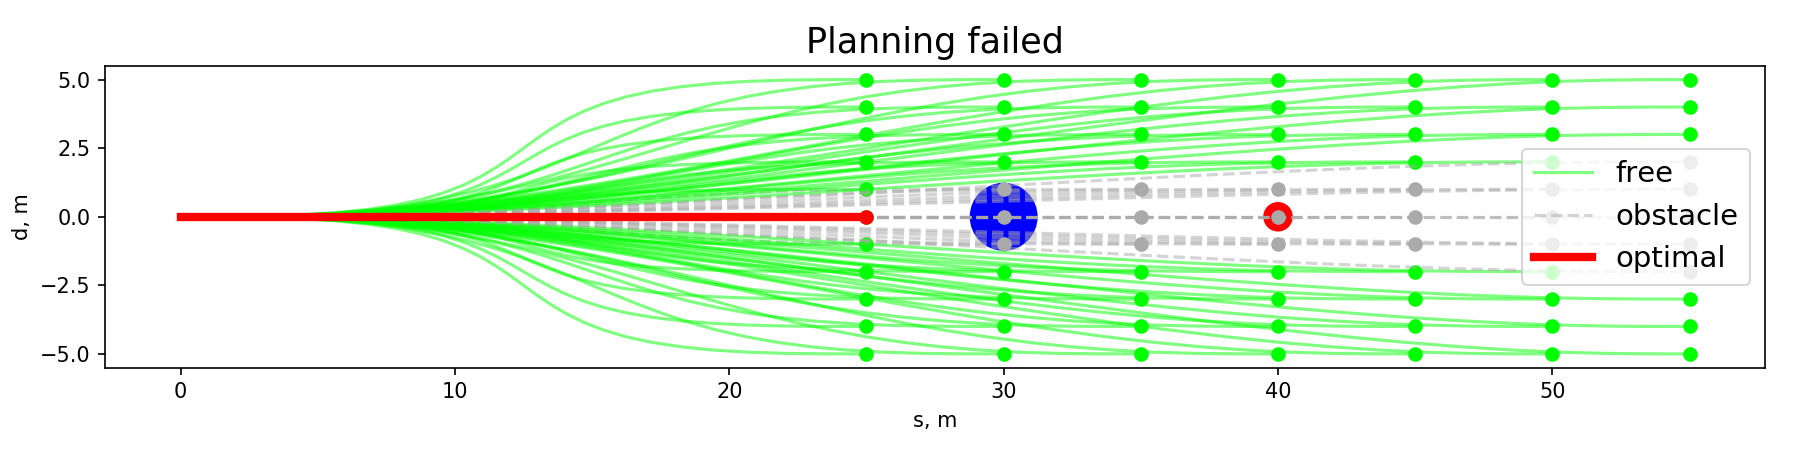
\includegraphics[width=\linewidth]{images/quintic_planning_failed} \\ а)
    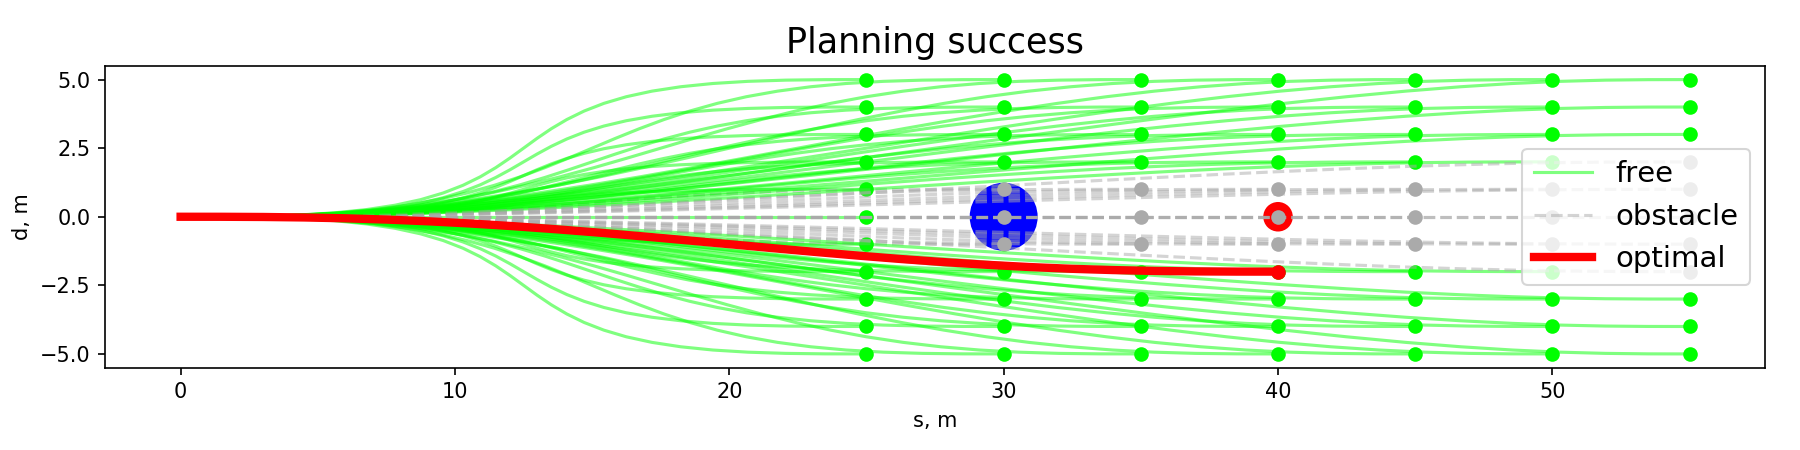
\includegraphics[width=\linewidth]{images/quintic_planning_success} \\ б)
    \caption{Пример планирования траектории с учетом препятствия при различных весовых коэффициентах:
    а) подходящая траектория не была найдена, б) подходящая траектория была найдена}
    \label{img:quintic_planning_failed}
\end{figure}

В результате экспериментальной проверки было установлено, что рассмотренный метод формирования программной траектории
обладает такими недостатками, как сильная зависимость от весовых коэффициентов функционалов стоимости и застревание
в локальном минимуме, т.е. метод формирует траектории, оптимальные в данный момент, но неоптимальные с точки зрения
достижения цели. Иллюстрация этой проблемы представлена на рисунке \ref{img:quintic_planning_failed}.

На рисунке изображена смоделированная ситуация. Автомобиль движется по дороге с постоянной скоростью, имеется локальная
цель с продольной координатой 40 м. Препятствие в форме окружности радиусом 1.5 м имеет продольную координату 30 м.
Для наглядности изображения осуществлялось варьирование только продольных и поперечных координат конечного состояния,
скорость и время маневра не изменялись. На рисунке изображены два результата планирования с различными весовыми
коэффициентами в функционале стоимости.

Для того, чтобы объехать препятствие, автомобиль должен отклониться от опорной траектории. Этот маневр приведет
к следующим изменениям в функционале стоимости \ref{eq:cost_lon}:
\begin{itemize}
      \item отклонение $d$ от опорной траектории увеличиться, что приведет к увеличению члена $K_dd(T)^2$;
      \item совершенные маневры приведут к увеличению $K_{dj}\int_{t_0}^{t_1}{\dddot{s}(t)^2dt}$;
      \item общее время маневра приведет к увеличению члена $K_{st}T$;
      \item автомобиль будет ближе к продольной цели, что приведет к уменьшению $K_s(s(T)-S_1)^2$
\end{itemize}

Итоговое значение функционала стоимости и принятое решение зависит от соотношения весовых коэффициентов $K_d$, $K_{dj}$,
$K_{st}$, $K_s$.

Эту проблему можно решить, если модифицировать алгоритм планирования движения путем осуществления нескольких шагов
планирования, т.е. рекурсивно запустить планирование повторно из каждого конечного состояния. Такой метод существенно
увеличит вычислительную сложность алгоритма, но позволит осуществлять планирование с большим горизонтом и осуществлять
более сложные маневры.

Поэтому была предложена модификация метода формирования программного движения, совмещающая планирование программного
движения метод интерполяции кривых с применением поиска кратчайшего пути на графе. В предложенном методе сначала
осуществляется построение графа возможных состояний, вершины которого получаются аналогично методу, описанному ранее,
т.е. путем варьирования конечного состояния: продольного и поперечного положения, продольной скорости и длительности
маневра. Затем осуществляется выбор вершины и пути к ней, которые минимизируют функционал стоимости. Для этого
функционал стоимости был переписан следующим образом, разделившись на стоимость вершины, описывающую, насколько это
состояния отдалено от целевого, и  стоимость пути на графе к этой вершине, описывающую маневры, которые необходимо
совершить для достижения этой вершины:

\begin{align}
    C_{move}  = &K_{lon}K_{sj}\int_{0}^{T}{\dddot{s}(t)^2dt} + K_{lat}K_{dj}\int_{0}^{T}{\dddot{d}(t)^2dt} \\
    C_{state} = &K_{lon}\Big[K_s \big(s(T) - S_1\big)^2 + K_v \big(\dot{s}(T) - \dot{S_1}\big)^2 + K_{st} T\Big] + \\
                &K_{lat}\Big[K_d d(T)^2 + K_{dt} T\Big] \nonumber
\end{align}

Поиск кратчайшего пути на графе осуществляется с помощью алгоритма Дейкстры. Пример формирования набора траекторий
представлен на рисунке \ref{img:multistep_trajectories}. Для наглядности осуществлялось варьирование только поперечных
конечных состояний.

\begin{figure}[h]
    \centering
    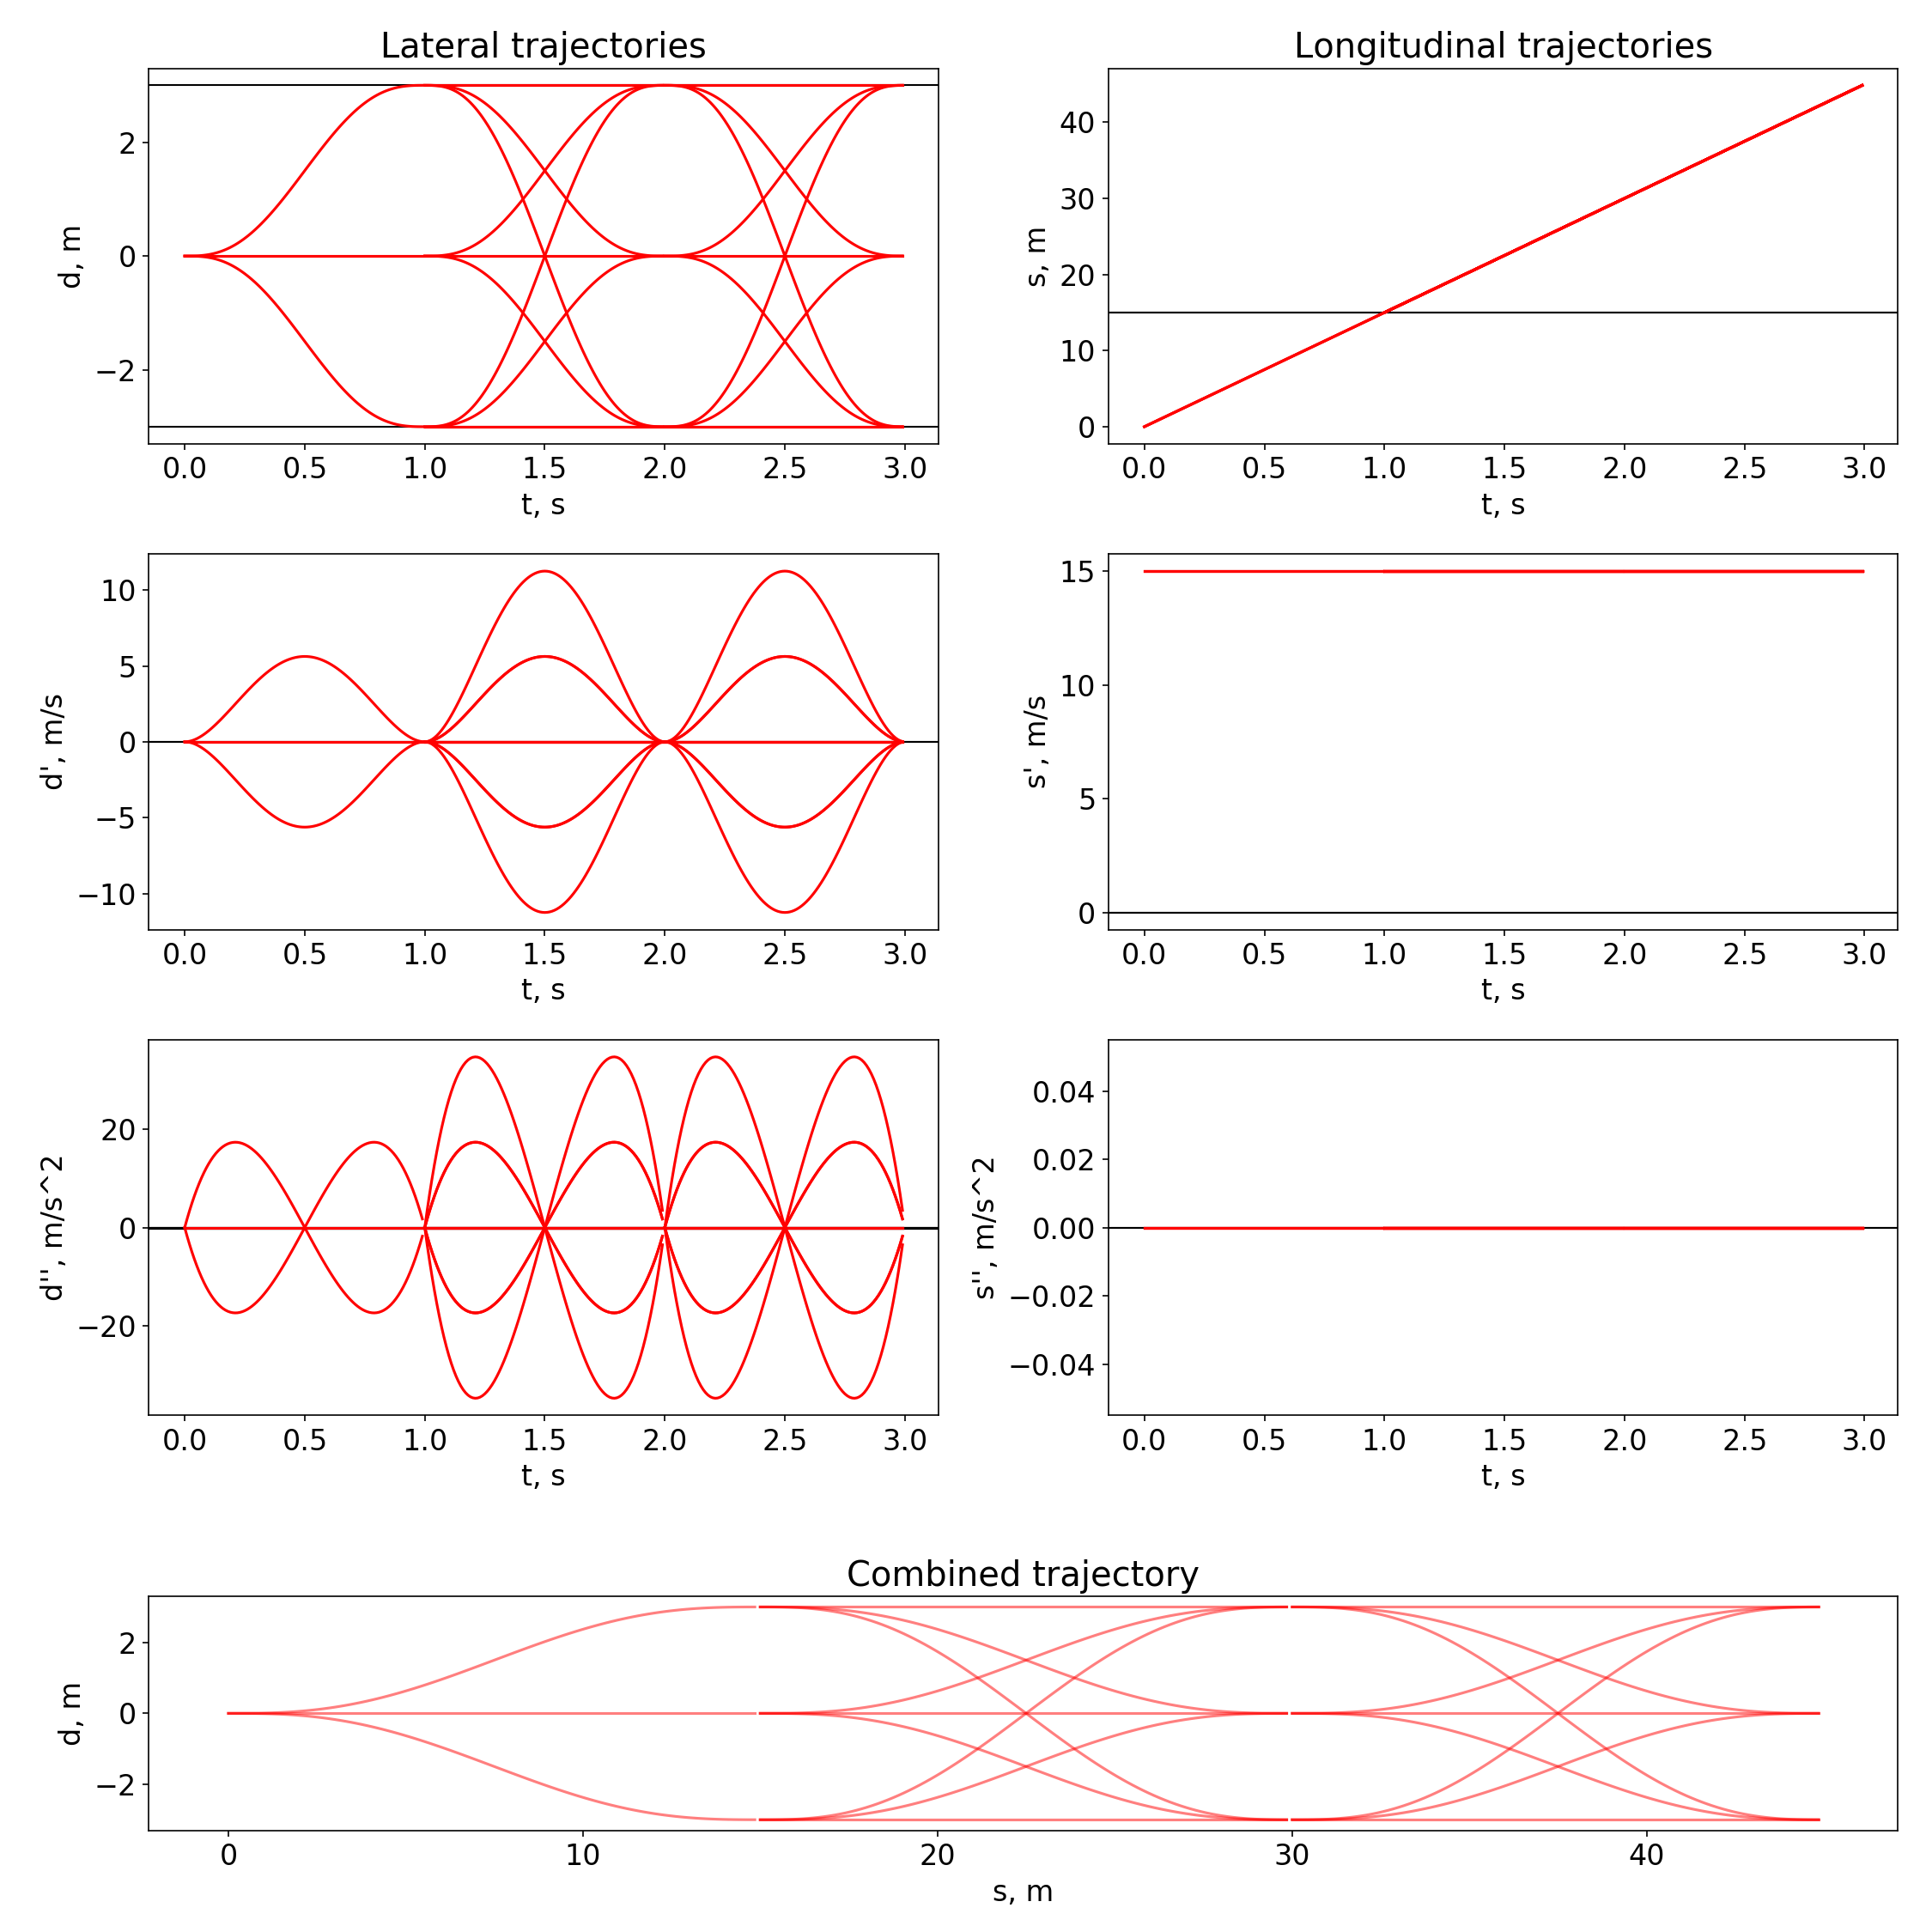
\includegraphics[width=\linewidth]{images/2_project/quintic_2/multistep_trajectories}
          \caption{Пример формирования набора траекторий}
    \label{img:multistep_trajectories}
\end{figure}

Для реализации рулевого управления с обратной связью применена упрощенная модель на базе
модель МакАдама.

Управляющий сигнал для рулевого управления получается с помощью пропорционального (П) регулятора
из угла между текущим направлением движения автомобиля (вектором скорости) и направлением на
точку траектории на некотором расстоянии впереди. Это позволяет учитывать будущие изменения
в траектории и реагировать на них заранее.

По причине того, что траектория представлена в виде большого количества плотно расположенных
точек, выбор необходимой точки осуществляется следующим образом: в начале находится ближайшая к автомобилю
точка на кривой, а затем от этой точки вперед по траектории перебираются точки, до тех пор, пока
расстояние от очередной точки до положения автомобиля не будет больше заданного (рисунок \ref{img:path_moving}).

\begin{figure}[h]
    \centering
    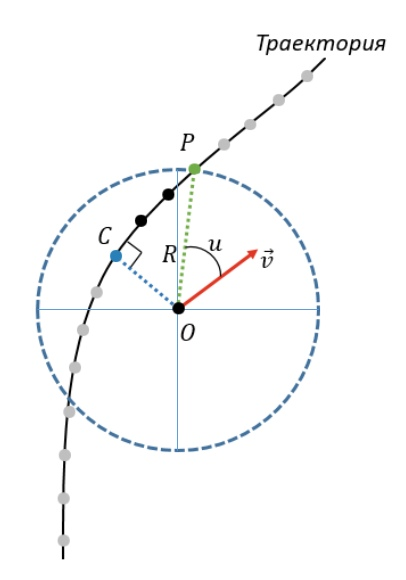
\includegraphics[width=0.4\textwidth]{images/path_moving}
    \caption{Пример формирования траекторий и выбора оптимальной}
    \label{img:path_moving}
\end{figure}


\textbf{В третьей главе} представлена реализация системы управления беспилотным автомобилем с
использованием подхода, описанной во второй главе.

Система управления построена на базе Robot Operation System (ROS) ~--- фреймворка для разработки
программного обеспечения для роботов. Использование ROS обладает большим количеством преимуществ
и существенно упрощает процесс разработки ПО:
\begin{itemize}
    \item модульная архитектура, основанная на нодах (nodes), позволяющая разрабатывать
          и тестировать отдельные модули системы независимо,
    \item встроенный удобный механизм межпроцессного взаимодействия (топики и сервисы),
    \item большое количество библиотек, реализующих распространенные в робототехнике алгоритмы,
    \item большое количество библиотек, реализующих работу с распространенным оборудованием,
    \item хорошая документация и сообщество.
\end{itemize}

Был реализован прототип системы управления беспилотным автомобилем и испытан на мобильной
колесной платформе, представленной на рисунке \ref{img:car}.

\begin{figure}[h]
    \centering
    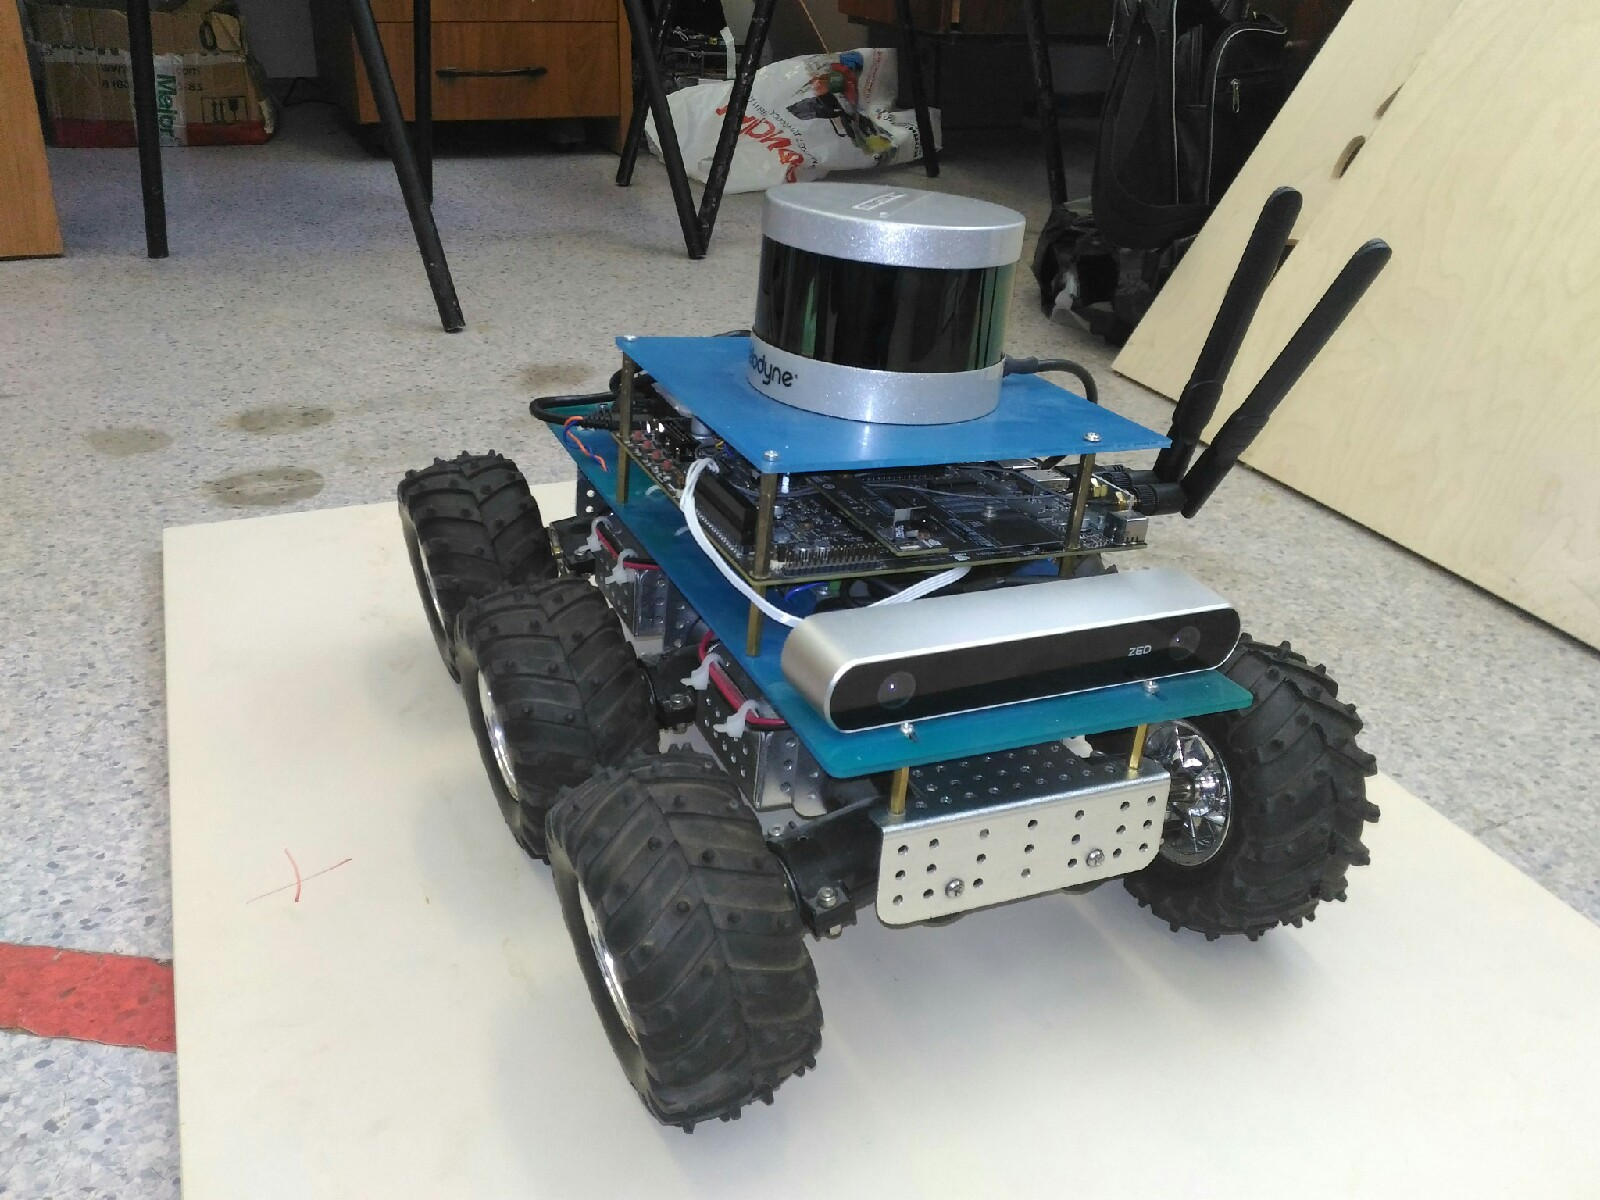
\includegraphics[width=0.5\textwidth]{images/car}
    \caption{Внешний вид колесной платформы}
    \label{img:car}
\end{figure}

В качестве бортового компьютера применена встраиваемая система NVidia Jetson TX2. На платформе размещены
стереокамера ZED Camera и LiDAR Velodyne VLP-16. Стереокамера используется для определения текущего локального
положения и ориентации платформы в пространстве с помощью SLAM-алгоритма, поставляемого с библиотекой
камеры. LiDAR используется для определения препятствий. Т.к. целью данной работы была разработка алгоритмов
движения, разработка полноценной системы компьютерного зрения не проводилась. Применен простейший алгоритм
обнаружения препятствий:
\begin{enumerate}
    \item в облаке точек осуществляется выделение плоскости с помощью алгоритма RANSAC,
    \item облако точек, получаемое от LiDAR разбивается с помощью двухмерной регулярной сетки,
    \item за препятствия считаются те клетки сетки, в который присутствует более определенного
          количества точек, отмеченные как выбросы (outliers);
    \item применяется трассировка пути с помощью алгоритма Брезенхема для растрирования линии, чтобы
          разделить пространство на свободные клетки до препятствия, клетки препятствия и клетки в неизвестном
          состоянии позади препятствия;
    \item происходит расширение препятствий путем растрирования круга определенного радиуса вокруг каждой
          клетки препятствий для учета габаритов мобильной платформы.
\end{enumerate}

Результат работы алгоритма приведен на рисунке \ref{img:obstacles_lidar}.

\begin{figure}[h]
    \centering
    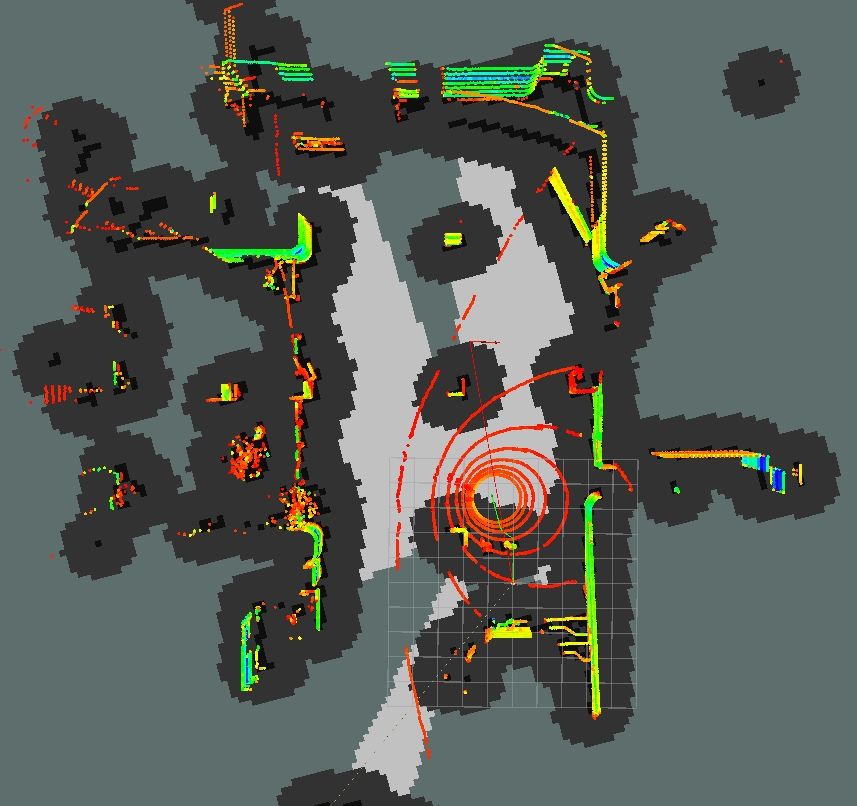
\includegraphics[width=\linewidth]{images/3_devel/obstacles_lidar}
    \caption{Результат работы алгоритма детектирования препятствий}
    \label{img:obstacles_lidar}
\end{figure}

Архитектура системы управления представлена на рисунке \ref{img:ros_arch}.

\begin{figure}[h]
    \centering
    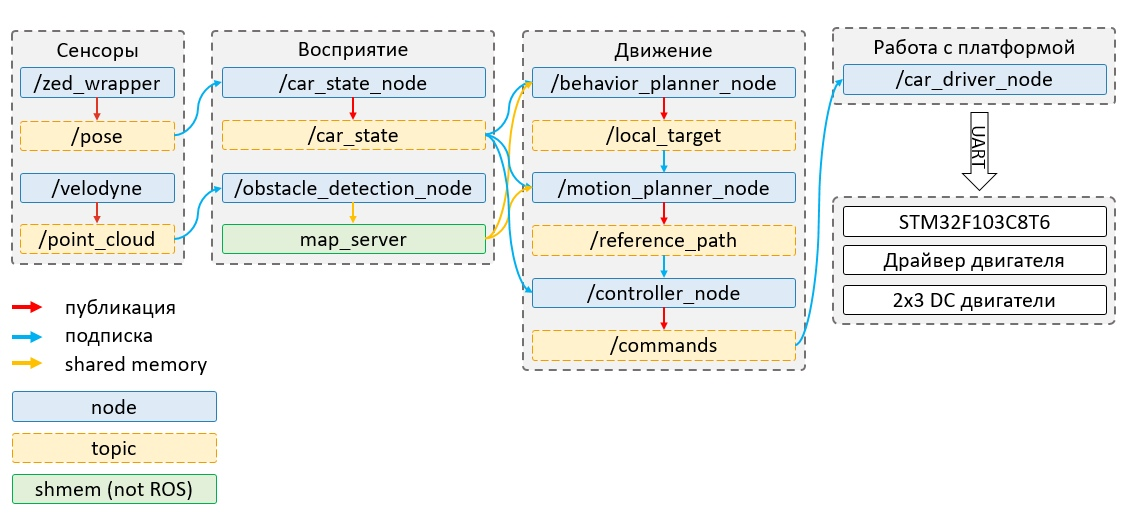
\includegraphics[width=\textwidth]{images/ros_arch}
    \caption{Мобильная платформа, используемая в экспериментах}
    \label{img:ros_arch}
\end{figure}

Система управления состоит из четырех основных блоков: блока работы с сенсорами, блока восприятия,
реализующего алгоритмы компьютерного зрения, блока управления движением, реализующего алгоритмы
планирования движения, и блока работы с платформой, управляющего двигателями.

Основными нодами являются motion\_planner\_node и controller\_node, реализующих локальное планирование
траектории и регулятор обратной связью соответственно.

\textbf{В четвертой главе} представлен анализ результатов работы. В рамках диссертационного исследования
была разработана и реализована система управления движением беспилотного автомобиля с использованием
представленного подхода. Алгоритм планирования движения основан на интерполяции траектории с помощью
полиномов пятого порядка, регулирование рулевого управления с обратной связью реализовано на основе
модель МакАдама.

Для оценки работы системы управления беспилотным автомобилем было проведено экспериментальное исследование
с помощью мобильной платформы. Поставленные задачи: определение точности следования по заданной траектории
с помощью регулятора с обратной связью и проверка работы алгоритма планирования траектории.

На рисунке \ref{img:path_moving_test} представлено сравнение программной (оранжевая линия)
и измеренной с помощью SLAM-алгоритма (синяя линия) траекторий при движении автомобиля по кругу.
Максимальное отклонение составило примерно 5 см.

\begin{figure}[h]
    \centering
    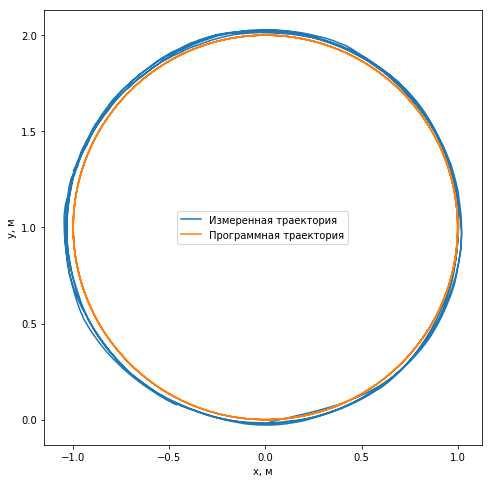
\includegraphics[width=0.7\textwidth]{images/path_moving_test}
    \caption{Движение по заданной траектории}
    \label{img:path_moving_test}
\end{figure}

На рисунке \ref{img:obstacle_avoidance} представлена визуализация движения с объездом статических
препятствий.

\begin{figure}[h]
    \centering
    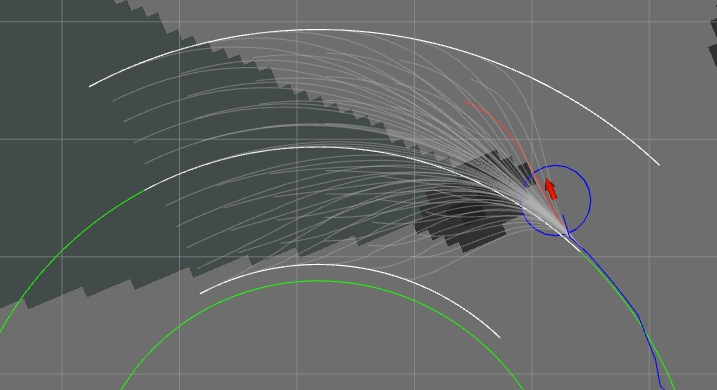
\includegraphics[width=0.7\textwidth]{images/obstacle_avoidance}
    \caption{Движение по заданной траектории}
    \label{img:obstacle_avoidance}
\end{figure}

Текущее положение и ориентация модели автомобиля, полученное с помощью SLAM-алгоритма, отмечено
красной стрелкой. Черным и темно-серым отмечены препятствие, определенное с помощью LiDAR и буферная
зона вокруг него соответственно. Зеленая линия отмечает идеальную траекторию, представляющую
середину дороги. В данном эксперименте идеальная траектория представляла собой спираль и считывалась
из файла, в реальности за формирование цели и идеальной траектории отвечает behaviour planner.
Белые линии отмечают виртуальные границы дороги. Многочисленные серые линии ~--- множество
сгенерированных траекторий-кандидатов. Красная линия ~--- выбранная оптимальная траектория
в объезд препятствия.



\textbf{В заключении} работы сформулированы общие выводы о значимости данной работы для
организации и перспективах исследования.

\referchapter{ОСНОВНЫЕ РЕЗУЛЬТАТЫ РАБОТЫ}
\begin{enumerate}
    \item Проведен анализ подходов к построению систем управления беспилотными
          автомобилями, определена общая архитектура и выделены общие блоки.
    \item Проведен анализ методов формирования программного движения применительно к беспилотным наземным транспортным
          средствам.
    \item Спроектирован и реализован прототип системы управления движением беспилотного
          наземного транспортного средства на базе мобильной колесной платформы.
    \item Проведены испытания на базе мобильной платформы, которые показали возможность
          реализованной системы планировать траекторию движения в объезд препятствий и
          точно следовать запланированной траектории с помощью обратной связи от камеры глубины.

\end{enumerate}

\referchapter{ПЕРСПЕКТИВНЫЕ НАПРАВЛЕНИЯ РАЗВИТИЯ РАБОТЫ}
Данная работа является начальным этапом в исследовании разработке системы управления
беспилотным автомобилем.
Дальнейшее улучшение возможностей системы построения программных траекторий может быть осуществлено путем использования
программы "ФРУНД" для проверки и/или формирования участков траектории с целью достижения лучшего учета динамических
ограничений транспортного средства.

Вторым направлением работ является исследование и разработка системы компьютерного зрения,
которая является важнейшим блоком в архитектуре управления беспилотным автомобилем.

\referchapter{ПУБЛИКАЦИИ ПО ТЕМЕ ДИССЕРТАЦИИ}
Опубликованные:
\begin{enumerate}
    \item Марков, А.Е. Проект системы компьютерного зрения для беспилотного автомобиля / А.Е. Марков, П.С. Тарасов
          // Смотр-конкурс научных, конструкторских и технологических работ студентов Волгоградского государственного
          технического университета (г. Волгоград, 16-20 апреля 2018 г.) : тез. докл. / редкол.: А. В. Навроцкий (отв. ред.)
          [и др.] ; Волгоградский гос. техн. ун-т, Совет СНТО. - Волгоград, 2018. - C. 166-167.
    \item  Марков, А.Е. Система управления беспилотным автомобилем / А.Е. Марков, П.С. Тарасов, Ан.В. Скориков //
           Прогресс транспортных средств и систем – 2018 : материалы междунар. науч.-практ. конф. (г. Волгоград,
           9-11 октября 2018 г.) / редкол.: И. А. Каляев, Ф. Л. Черноусько, В. М. Приходько [и др.] ; ВолгГТУ, РФФИ,
           «ФНПЦ «Титан–Баррикады». - Волгоград, 2018. - C. 206.
\end{enumerate}

\bigskip
Поданные на публикацию:
\begin{enumerate}
    \item Система движения по заданной траектории для беспилотного автомобиля / А. Е. Марков [и др.]
\end{enumerate}


\end{document}